\section{Proof of Proposition \ref{prop:scheme_sr_sgc_straggler_tolerance}}\label{app:proof_scheme_B_straggler_tolerance}

Consider a straggler pattern which conforms to either (i) the $(B,W,\lambda)$-bursty straggler model or else, (ii) the $s$-stragglers-per-round model, in any window of rounds $W_j\triangleq[j:j+W-1]$, $j\in[1:J+T-W+1]$. Let $t'\in[1:J+T]$ denote the first round in which there are more than $s$ stragglers. All the tasks attempted in round-$t'$ correspond to job-$t'$. By assumption, the straggler pattern, when restricted to the $W$ rounds $[t':t'+xB]$ conforms to the $(B,W,\lambda)$-bursty straggler model. Let there be $\lambda_0>s$ stragglers in round-$t'$. In round-$(t'+B)$, $\lambda_0-s$ tasks corresponding to job-$t'$ will be attempted by $\lambda_0-s$ workers who were stragglers in round-$t'$ (see Figure~\ref{fig:sr_sgc_scheme}). Because of the straggler model assumption, none of these workers will be stragglers again in round-$(t'+B)$ and hence, job-$t'$ will be finished in round-$(t'+B)$ with delay $B$. Clearly, round-$(t'+B)$ is a ``deviation'' from the $(n,s)$-GC scheme as not all tasks in this round correspond to job-$(t'+B)$. Suppose now there are $\lambda_1$ stragglers in round-$(t'+B)$. Thus, number of task results corresponding to job-$(t'+B)$ returned by workers in round-$(t'+B)$ is given by $n-\lambda_1-\lambda_0+s$. If this quantity is greater than or equal to $n-s$, job-$(t'+B)$ can be finished in round-$(t'+B)$ itself and there will be a ``reset'' in round-$(t'+2B)$ as all tasks there correspond to job-$(t'+2B)$. On the other hand, if $(n-\lambda_1-\lambda_0+s)<(n-s)$, $(\lambda_0+\lambda_1-2s)$ tasks corresponding to job-$(t'+B)$ will be attempted in round-$(t'+2B)$ by workers who did not return task results corresponding to job-$(t'+B)$ in round-$(t'+B)$. These workers can either be stragglers in round-$(t'+B)$ or else, be processing tasks corresponding to job-$t'$ in round-$(t'+B)$. In either case, these workers cannot be stragglers in round-$(t'+2B)$ owing to the straggler model (see Figure~\ref{fig:sr_sgc_scheme}). Hence, job-$(t'+B)$ will finish in round-$(t'+2B)$ will delay $B$. Now, if not enough task results corresponding to job-$(t'+2B)$ are returned in round-$(t'+2B)$, the minimum-required number of additional tasks corresponding to this job will be attempted in round-$(t'+3B)$ and so on. We will now show that there exist an $\ell\in[1:x]$ such that jobs $t',t'+B,\ldots,t'+(\ell-1)B$ are finished with delay precisely $B$ and job-$(t'+\ell B)$ is finished with delay $0$. i.e., there is a reset happening in round-$(t'+(\ell+1)B)$. In order to show this, assume that jobs $t',t'+B,\ldots,t'+(x-1)B$ have some of their tasks attempted with delay $B$ (i.e., no reset in rounds $t'+2B,\ldots,t'+xB$). Because of the straggler model, all these delayed tasks are guaranteed to succeed and hence all these jobs finish with delay $B$. We should now prove that there is a reset in round-$(t'+(x+1)B)$, i.e., $\ell=x$. For $j\in[0:x]$, let $\lambda_j$ indicate the number of stragglers in round-$(t'+jB)$. Number of tasks corresponding to job-$(t'+(x-1)B)$ attempted in round-$(t'+xB)$ is given by $\lambda_0+\lambda_1+\cdots+\lambda_{x-1}-xs$. Thus, number of task results corresponding to job-$(t'+xB)$ received by master in round-$(t'+xB)$ is given by:
\begin{eqnarray}n n-\lambda_x-(\lambda_0+\lambda_1+\cdots+\lambda_{x-1}-xs)&=&n-\lambda_0-\lambda_1-\cdots-\lambda_x+xs\\
&\geq& n-\lambda+xs\\
&\geq&n-\lceil\frac{\lambda}{x+1}\rceil(x+1)+xs\\
&=&n-s(x+1)+xs\\
&=& n-s,
\end{eqnarray}
where we have used the fact that $\lambda_0+\cdots+\lambda_x\leq \lambda$ owing to the straggler model. Hence, in summary, we have showed that if all of jobs $t',t'+B,\ldots,t'+(x-1)B$ finish with delay $B$, then $t'+xB$ finishes with delay $0$ and there will be a reset in round-$(t'+(x+1)B)$. Thus, there exist $\ell\in[1:x]$ such that all jobs $t',t'+B,\ldots,t'+(\ell-1)B$ finish with delay $B$ and 
job-$(t'+\ell B)$ finishes with delay $0$. Because of the reset happening in round-$(t'+(\ell+1)B)$, the ``effect'' of Algorithm \ref{alg:constr_sr_sgc} is now confined only to rounds $t',t'+B,\ldots,t'+\ell B$. We can now safely regard rounds  $t',t'+B,\ldots,t'+\ell B$ as straggler-free as these rounds contain only tasks corresponding to jobs $t',t'+B,\ldots,t'+\ell B$ and  we have shown that all these jobs succeed with delay at most $B$. We can now essentially repeat all these steps starting with finding the next ``first'' round-$t'$ having more than $s$ stragglers. After repeating these arguments sufficient number of times, eventually, we will be left with jobs $R\subseteq [1:J]$, where all rounds in $R$ has at most $s$ stragglers. Workers in each round-$r$, $r\in R$, attempt only tasks corresponding to job-$r$. Thus, all these jobs can be finished with delay $0$. This completes the proof.

\begin{figure*}
		\centering
		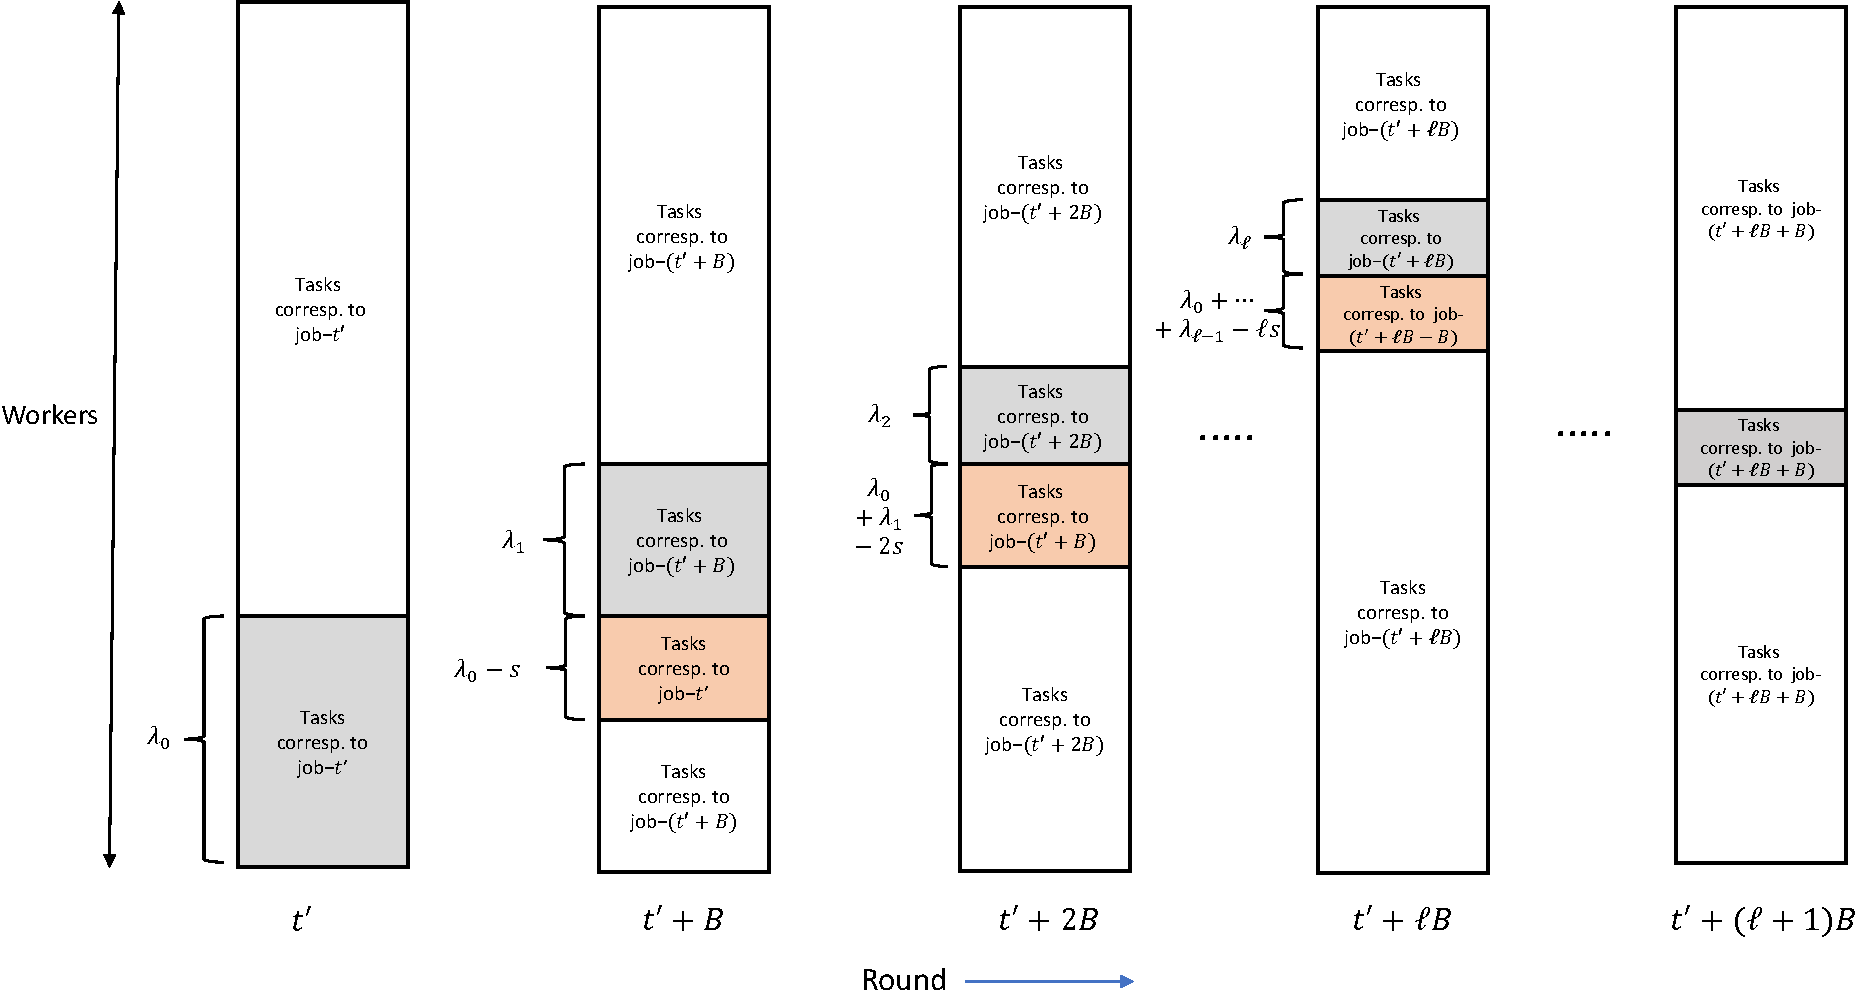
\includegraphics[scale=0.44]{figs/ch2/fig_SR_SGC_v2}
		\caption{An illustration of task assignment in SR-SGC. In the initial rounds, the task assignment is precisely as in an $(n,s)$-GC scheme and all tasks in round-$t$ correspond to job-$t$.  In any such round-$t$, if there are at most $s$ stragglers, job-$t$ can be finished in round-$t$ itself. Let $t'$ denote a round where all tasks correspond to job-$t'$ and there are $\lambda_0>s$ stragglers. Stragglers are indicated in grey color. In round-$(t'+B)$, there is a deviation from the $(n,s)$-GC scheme as $\lambda_0-s$ tasks corresponding to job-$t'$ will be attempted in this round (these tasks which are attempted with delay $B$ are indicated in orange). These tasks are attempted by workers who did not return task results corresponding to job-$t'$ in round-$t'$. In round-$(t'+B)$, $n-\lambda_1-\lambda_0+s$ workers return task results corresponding to job-$(t'+B)$. If this quantity is lesser than $n-s$, $\lambda_0+\lambda_1-2s$ tasks corresponding to job-$(t'+B)$ will be attempted in round-$(t'+2B)$ by workers who did not return task results corresponding to job-$(t'+B)$ in round-$(t'+B)$. The process is continued in a similar manner. If the straggler pattern in the window of rounds $[t':t'+xB]$ conforms to the $(B,W,\lambda)$-bursty straggler model, there exists an $\ell\in[1:x]$ such that in round-$(t'+(\ell+1)B)$ a ``reset'' happens back to the $(n,s)$-GC scheme, i.e., in round-$(t'+(\ell+1)B)$ all tasks correspond to job-$(t'+(\ell+1)B)$.}
		\label{fig:sr_sgc_scheme}
\end{figure*}

\clearpage

\section{Proof of Proposition \ref{prop:scheme_m_sgc_straggler_tolerance}}\label{app:proof_of_working_constr_b_sgc}


Consider the computation of $g(t)$, $t\in[1:J]$ in the presence of a straggler pattern conforming to one of the following; (i) $(B,W,\lambda)$-bursty straggler model or else, (ii) $(N=B,W'=W+B-1,\lambda'=\lambda)$-arbitrary straggler model. By design of Algorithm \ref{alg:constr_b_sgc}, for each worker-$i$, mini-tasks $\{\mathcal{T}_i(t;0),\mathcal{T}_i(t+1;1),\ldots,\mathcal{T}_i(t+W-2+B;W-2+B)\}$ correspond to job-$t$. Master has to compute:
\begin{equation*}
g(t)\triangleq \underbrace{\sum_{j\in[0:(W-1)n-1]}g_{j}(t)}_{g'(t)}+\underbrace{\sum_{l\in[(W-1)n:(W-1+B)n-1]}g_{l}(t)}_{g''(t)}
\end{equation*}
by the end of round-$(t+T)$, where $T= W-2+B$. If $\lambda=n$, we only have the $g'(t)$ part and set $g''(t)\triangleq 0$. We will now show that master will be able to compute each of $\{g'(t),g''(t)\}$ individually by the end of round-$(t+W-2+B)$ in presence of straggler patterns conforming to one of these straggler models. 

\textit{Computing $g'(t)$}: From Algorithm \ref{alg:constr_b_sgc}, it can be noted that mini-task $\mathcal{T}_i(t+j;j), j\in[0:W-2]$ involves computing $g_{i(W-1)+j}(t)$. If worker-$i$ is not a straggler in all the rounds $[t:t+W-2]$, clearly, master can compute $\sum_{j\in [0:W-2]}g_{i(W-1)+j}(t)$ in the end of round-$(t+W-2)$.

Now, consider the remaining situation that worker-$i$ is a straggler in at least one of the rounds within $[t:t+W-2]$. We initially discuss the case that the straggler pattern conforms to $(B,W,\lambda)$-bursty straggler model. Worker-$i$ experiences at most $B$ straggling rounds (see Figure~\ref{fig:burst_model_distr_stragglers}) among rounds $[t:t+W-2+B]$. Suppose worker-$i$ is a straggler in $x'$ rounds, $x'\in[1:B]$, within rounds $[t:t+W-2]$. Thus, $x'$ partial gradients among $\{g_{i(W-1)+j}(t)\}_{j\in[0:W-2]}$ are not returned by worker-$i$ in rounds $[t:t+W-2]$. However, Algorithm \ref{alg:constr_b_sgc} reattempts those failed partial gradient computations in rounds $[t+W-1:t+W-2+B]$. Even if there are $B-x'$ straggling rounds among $[t+W-1:t+W-2+B]$, in the remaining $x'$ rounds, the failed partial gradients will be successfully computed. Hence, using mini-task results returned by worker-$i$, master can compute $\sum_{j\in [0:W-2]}g_{i(W-1)+j}(t)$ by the end of round-$(t+W-2+B)$. By accumulating results from all the $n$ workers, master will be able to compute $g'(t)$ by the end of round-$(t+W-2+B)$.


\begin{figure*}[b]
	\centering
	\subfloat[]{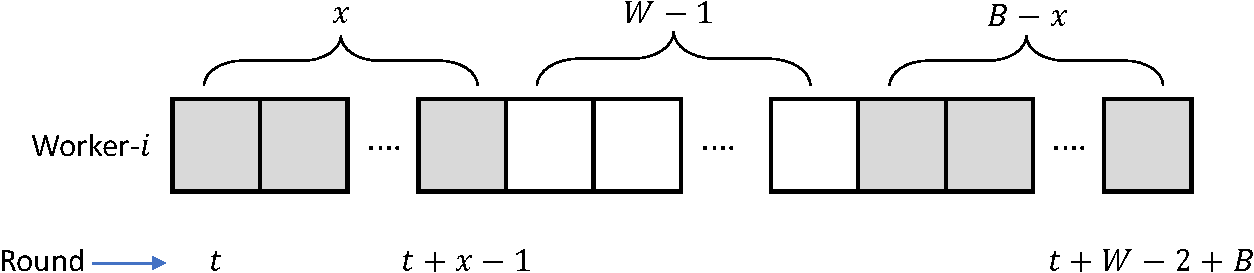
\includegraphics[width=8cm]{figs/ch2/fig_proof_of_working_B_SGC_1}}
	\ \ \ \ \ \subfloat[]{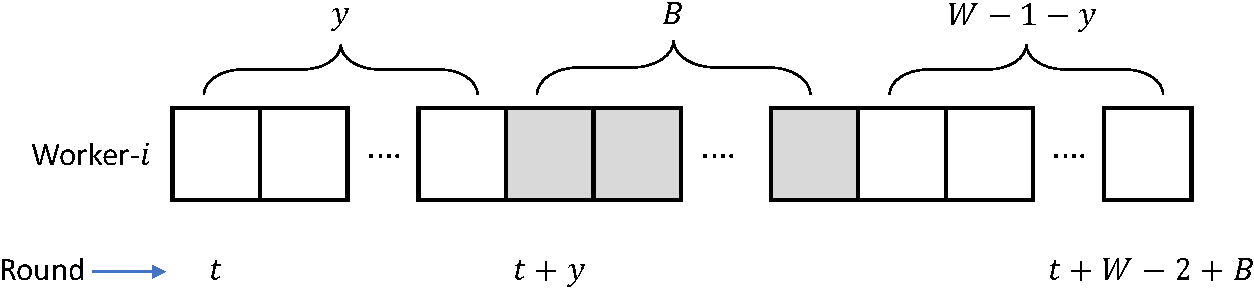
\includegraphics[width=8cm]{figs/ch2/fig_proof_of_working_B_SGC_2}}
	\caption{In the figure, shaded boxes depict straggling rounds. Consider a straggler pattern conforming to the $(B,W,\lambda)$-bursty straggler model. The straggling rounds, if any, seen by worker-$i$ among rounds $[t:t+W-2+B]$ will be a subset of the $B$ straggling rounds indicated in either situation (a) or (b). Here $x\in[1:B]$, $y\in[0:W-1]$.}\label{fig:burst_model_distr_stragglers}
\end{figure*}


We now consider the case where straggler pattern conforms to the  $(N=B,W'=W+B-1,\lambda'=\lambda)$-arbitrary straggler model. As per the model, a worker can be a straggler in at most $N=B$ rounds in any sliding window consisting of $W'=W-1+B$ consecutive rounds. Let worker-$i$ be a straggler in $x''$ rounds ($x''\in[1:B]$) within rounds $[t:t+W-2]$ and at most $B-x''$ rounds within $[t+W-1:t+W-2+B]$. Clearly, $x''$ mini-tasks among $\{g_{i(W-1)+j}(t)\}_{j\in[0:W-2]}$ fail in their first attempt. However, as worker-$i$ is a non-straggler in at least $x''$ rounds within $[t+W-1:t+W-2+B]$, these mini-tasks will eventually be repeated and  finished. Thus, master computes $\sum_{j\in [0:W-2]}g_{i(W-1)+j}(t)$ by the end of round-$(t+W-2+B)$. Collecting results from all the $n$ workers, master will be able to compute $g'(t)$ by the end of round-$(t+W-2+B)$.


\textit{Computing $g''(t)$}: Again, we begin with discussing the case where a straggler pattern conforms to the $(B,W,\lambda)$-bursty straggler model. For any straggler pattern  conforming to this straggler model, there exist $(n-\lambda)$ workers who do not have any straggling rounds among any window of rounds of the form $W_j\triangleq [j:j+W-1]$. In particular, consider the rounds in $W_{t}$. Assume that worker-$i$ does not have any straggling rounds in the window $W_t$. Thus, mini-tasks $\{\mathcal{T}_i(t+l;l)\}_{l=0}^{W-2}$ will be successful and partial gradients $\{g_{i(W-1)+l}(t)\}_{l=0}^{W-2}$ will be computed in the first attempt. Hence, from Algorithm \ref{alg:constr_b_sgc}, it can be inferred that the mini-task $\mathcal{T}_i(t+W-1;W-1)$ involves computing $\ell_{i,0}(t)$. As worker-$i$ is not a straggler in round-$(t+W-1)$, master receives the linear combination $\ell_{i,0}(t)$. As there are $(n-\lambda)$ such workers returning $\ell_{i,0}(t)$'s, owing to the use of $(n,\lambda)$-GC, master can compute $\sum_{l\in[(W-1)n:Wn-1]}g_{l}(t)$ by the end of round-$(t+W-1)$. Similarly, due to the $(B,W,\lambda)$-bursty straggler model assumption, there are $(n-\lambda)$ workers who do not have any straggling rounds in the window $W_{t+1}=[t+1:t+W]$. Let worker-$i'$ be one such worker. All the mini-tasks $\{\mathcal{T}_{i'}(t+1;1),\cdots,\mathcal{T}_{i'}(t+W-2;W-2)\}$ will be successful and  $\{g_{i'(W-1)+l}(t)\}_{l=1}^{W-2}$ will be computed in their first attempts. In round-$t$, worker-$i'$ can possibly be a straggler. However, as worker-$i'$ is not a straggler in round-$(t+W-1)$, the failed computation of  $g_{i'(W-1)}(t)$ will be reattempted and finished in round-$(t+W-1)$. Thus, by the end of round-$(t+W-1)$, all partial gradients $\{g_{i'(W-1)+l}(t)\}_{l=0}^{W-2}$  are guaranteed to be computed. Hence, mini-task $\mathcal{T}_{i'}(t+W;W)$ involves computing $\ell_{i',1}(t)$. As round-$(t+W)$ is a non-straggling round, master will receive $\ell_{i',1}(t)$ in the end of round-$(t+W)$. Using $(n-\lambda)$ such $\ell_{i',1}(t)$'s, master can compute $\sum_{l\in[Wn:(W+1)n-1]}g_{l}(t)$. In a similar manner, it can be argued that, for $m\in[0:B-1]$, master will be able to compute $\sum_{l\in[(W-1+m)n:(W+m)n-1]}g_{l}(t)$ in the end of round-$(t+W-1+m)$. Hence, by the end of round-$(t+W-2+B)$, master is able to compute $g''(t)$.


In the case if straggler pattern conforms to the $(N=B,W'=W+B-1,\lambda'=\lambda)$-arbitrary straggler model, there are $n-\lambda$ workers who do not have any straggling rounds in $[t:t+W-2+B]$. For any such worker-$i$, computations of $\{g_{i'(W-1)+l}(t)\}_{l=0}^{W-2}$  are all finished by the end of round-$(t+W-2)$. Hence, in round-$(t+j)$, $j\in[W-1:W-2+B]$, worker-$i$ will compute and return $\ell_{i,j-W+1}(t)$ to master. Using $(n,\lambda)$-GC, results from $n-\lambda$ such workers can be used by master to obtain  $\sum_{l\in[jn:(j+1)n-1]}g_{l}(t)$.  Thus, by the end of round-$(t+W-2+B)$, master is able to compute $g''(t)$. 

